\documentclass{ctexart}
\usepackage[utf8]{inputenc}
\usepackage{graphicx}
\usepackage{tikz}
\usetikzlibrary{shapes,arrows}


\title{项目作业:五则运算计算器的实现}
\author{陈科辉 Keiver Pabula}
\date{30 December,2022}
\begin{document}
\maketitle

\section{设计思路}
首先我做了4个函数:

1. priority()函数:用于判断运算符的优先级;

2. transform()函数:将中缀表达式转化为后缀表达式;

3. op()函数:为了后续将符号和数字配在一起,将栈顶的两个数取出num1 num2,并在栈中删除

4. Caculator()函数:计算后缀表达式向量的末尾。

对于第一个函数它将五个运算符进行分级:+,-为1级; *,/为2级; $\^$为3级。他后续的作用是用于后续将中缀表达式转化为后缀表达式时决定运算符需要入栈还是直接放在后缀表达式后方。

对于第二个函数将中缀表达式转化为后缀表达式:它的方法首先判断表达式是否有输入错误,并且如果是-x或+x就默认其为0-x和0+x;然后循环整个表达式,将运算符放入根据上述的分级来判定运算符是否入栈,其次看是否有错误的表达式,例如除数为0,底数为0,括号不匹配…… 所以用case,只在(, ), /, $\^$的地方有不同其余都直接根据优先级分配,对于运算数全部都放入后缀表达式向量中,剩余的运算符也都放进去。

总结第二个函数:
在后缀表达式向量中将运算数放入,后放入运算符,而运算符放入的原则就是栈不为空,且运算符优先级小于等于栈顶元素优先级,则栈顶元素放在向量后方,栈顶元素也依次删除; 反之则将运算符入栈; 如果栈为空,或运算符等于'(',或栈顶元素为'('则直接入栈; 若当前运算符等于')',则将栈顶元素出栈置于后缀表达式尾, 直到遇到运算符'('。

第三个函数是用于取出后缀表达式排序后,数字栈最顶上的两个数字取出并删除,为了使后面可以搭配运算符直接计算。

第四个函数就是计算后缀表达式,方法就是从前到后依次取向量中的元素,如果是数则先将它从str转成double存入数字栈储存,然后当遇到运算符时就将数字栈中的最顶上两个元素取出,进行相对应的运算,得到的结果重新插入栈顶部;不断循环直到结束所有向量中的元素。(注意:除法除数不等于0,如果错了这里会报错)最后所剩的数字栈顶部的元素就是结果返回其值。


\section{测试结果}
简单的5个运算:
\begin{center}
  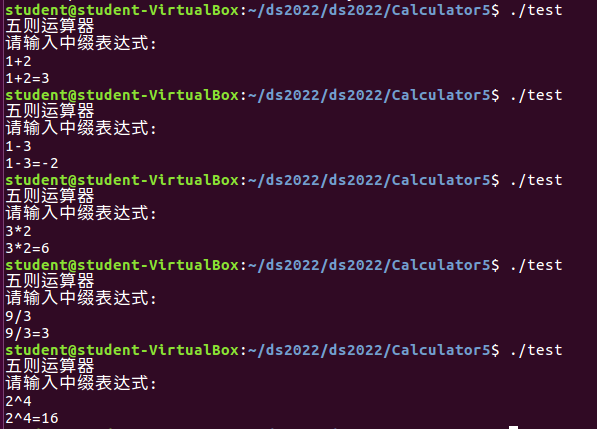
\includegraphics[scale=0.6]{ss1.png}
  \hspace{0.1in}
\end{center}
4个所给的算例:
\begin{center}
  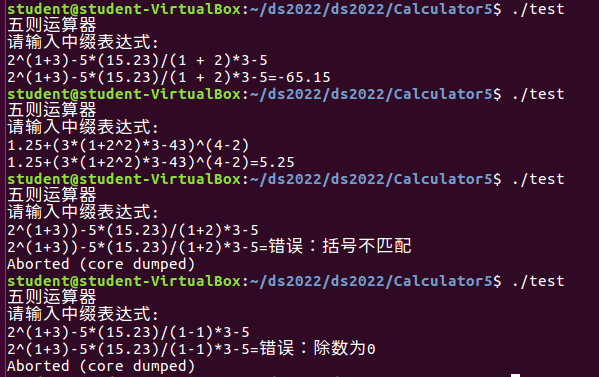
\includegraphics[scale=0.5]{ss2.png}
  \hspace{0.1in}
\end{center}
可以看到已经符合要求,且可以得到正确的答案。
\end{document}
